\documentclass[UTF8,a4paper,10pt]{ctexart}
\usepackage[margin=19mm,top=20mm,bottom=19mm]{geometry}
\usepackage{amsmath,amssymb,booktabs,tabularx,graphicx,xcolor,fancyhdr,enumitem,tikz}
\usetikzlibrary{arrows.meta,positioning}
\usepackage[colorlinks=true,linkcolor=teal,urlcolor=teal]{hyperref}
\definecolor{ink}{HTML}{142B43}\definecolor{accent}{HTML}{168579}
\pagestyle{fancy}\fancyhf{}\fancyhead[L]{\small CF2026 Project 1}\fancyhead[R]{\small 青序量化研究平台}
\fancyfoot[L]{\scriptsize 平台 V4 / v2.2.0 / 2026-09-22 · 固定历史快照 · 描述性结果}\fancyfoot[R]{\thepage/10}
\setlength{\headheight}{14pt}\setlength{\parskip}{4pt}\setlength{\emergencystretch}{2em}\setlength{\parindent}{2em}
\setlist{nosep,leftmargin=1.7em}\ctexset{section={format=\Large\bfseries\color{ink}},subsection={format=\normalsize\bfseries\color{accent}}}
\newcommand{\lead}[1]{\noindent{\bfseries\color{accent}#1}\par}
\newcommand{\page}[1]{\newpage\section*{#1}}
\begin{document}
\begin{center}{\small\color{accent}COMPUTATIONAL FINANCE / PROJECT 1}\\[8pt]
{\Huge\bfseries\color{ink}青序量化研究平台}\\[8pt]
{\Large 策略研究、风险分析与可扩展工作台}\\[8pt]
2026年9月22日\quad V4平台增强\quad 最终提交报告
\end{center}
\section*{1\quad 目标与主要结果}
\lead{从购买力目标升级为扣费后超过沪深300，同时保留选择失败与全部候选。}
平台覆盖数据质量、因子、横截面诊断、含费用回测、独立账本和可复现交付。用户将策略目标改为战胜沪深300。策略研究固定1,000股历史池及2025-01-02至2026-09-18区间，预先限定8个候选，比较经济主题、年度滚动Ridge、年度滚动LightGBM及固定融合。

当前默认策略为\textbf{年度滚动LightGBM＋波动预算}，用24个标准化/中性化输入预测股票相对排序，50只目标持仓，每20个交易日调仓，允许现金、不用杠杆。
\begin{center}\begin{tabular}{lr}\toprule
2025--2026固定417日历史区间 & 结果\\\midrule
累计净收益 / 年化净收益 & 25.13\% / 14.51\%\\
最大回撤 / 年化Sharpe & 9.88\% / 1.255\\
沪深300价格指数 / 全收益指数 & 14.55\% / 19.94\%\\
超过价格指数 / 全收益指数 & 10.58 / 5.19个百分点\\
交易费用 / 平均现金 & 24,506.76元 / 17.87\%\\\bottomrule
\end{tabular}\end{center}
\textbf{本段历史同时超过价格指数和含红利再投资的全收益指数。}双倍交易费用仍收益22.48\%，信号延后一日收益27.31\%。2023起连续运行累计44.09\%、最大回撤19.70\%，但2024年度落后价格指数7.28个百分点，不能声称每年都战胜市场。

\subsection*{选择边界必须与结果一起阅读}
V3验证期预选的价值质量组合在2025--2026仅收益4.30\%，没有超过指数。当前LightGBM是在查看本轮历史结果后，从通过验证净收益、超额收益和回撤门槛的候选中选出。V2已经看过同一最终区间，本次\textbf{不是独立盲测成功}。保留失败预选和8个候选，下一步应冻结规则做新数据前向验证。
\subsection*{平台增强版的实际能力}
研究总览汇集结果与入口；同区间策略对比支持版本、日期和基准选择；风险透镜提供月历、回撤恢复、60日滚动风险和静态现金情景；因子、行情与实验档案支持追查样本和订单。本版增强工具和可复现性，保留V3策略参数及历史选择边界，未把界面升级包装成新的独立验证。
\page{2\quad 软件结构与研究工作台}
\lead{数据、信号、组合、成交和分析分别维护，界面与命令行调用同一核心。}
\begin{center}\begin{tikzpicture}[node distance=4mm, every node/.style={draw=accent,fill=accent!5,rounded corners=1mm,align=center,text width=32mm,minimum height=13mm,font=\small}]
\node(a){数据快照\\字段/质量};\node(b)[right=of a]{因子/模型\\日期$\times$资产分数};\node(c)[right=of b]{组合/风险\\权重与现金};\node(d)[right=of c]{成交/分析\\账本与证据};
\draw[-{Stealth},accent](a)--(b);\draw[-{Stealth},accent](b)--(c);\draw[-{Stealth},accent](c)--(d);
\end{tikzpicture}\end{center}
\begin{center}\small\begin{tabularx}{\textwidth}{lX}\toprule
模块 & 职责与稳定接口\\\midrule
data / incremental & 行情及交易日、字段校验、幂等更新与数据身份。\\
factors / features / models & 日期$\times$资产分数；因子卡、可见财报与年度模型。\\
risk / engine & 目标权重、现金和成交约束；订单、成交、持仓及日账本。\\
analytics / strategies & 指标、独立核对、同区间分析与不可变策略版本。\\
界面 / CLI / 导出 & 共用核心；筛选、图表、参数实验和研究记录。\\\bottomrule
\end{tabularx}\end{center}
\subsection*{四项可直接使用的增强工具}
\begin{enumerate}
\item \textbf{策略对比：}最多五版策略，统一日期与价格/全收益基准，展示相对净值、风险、费用和相关性，导出CSV及计算假设。
\item \textbf{风险透镜：}月收益、下行风险、最深回撤及恢复日期；查看现金、换手和费用，交互分析静态现金配置与通胀假设。
\item \textbf{因子与行情：}12因子独立入口、日期诊断与样本查询；K线及成交量追查异常，缺原始数据时明确可用边界。
\item \textbf{实验档案：}按运行、日期、资产及订单状态筛选，查看参数、成交与账本，保存关联实验的本地研究笔记。
\end{enumerate}
\subsection*{公开证据与本地数据各有用途}
聚合日账本足以运行策略对比、风险诊断和结果导出，无Token也能离线展示真实历史结果。逐股行情、训练缓存和交易明细依赖本机快照；缺少时说明状态。每次参数回放保存新的运行目录，策略切换清除旧图，不混用旧结果。新增模型只需输出统一分数，新增分析以DataFrame作为输入。
\begin{center}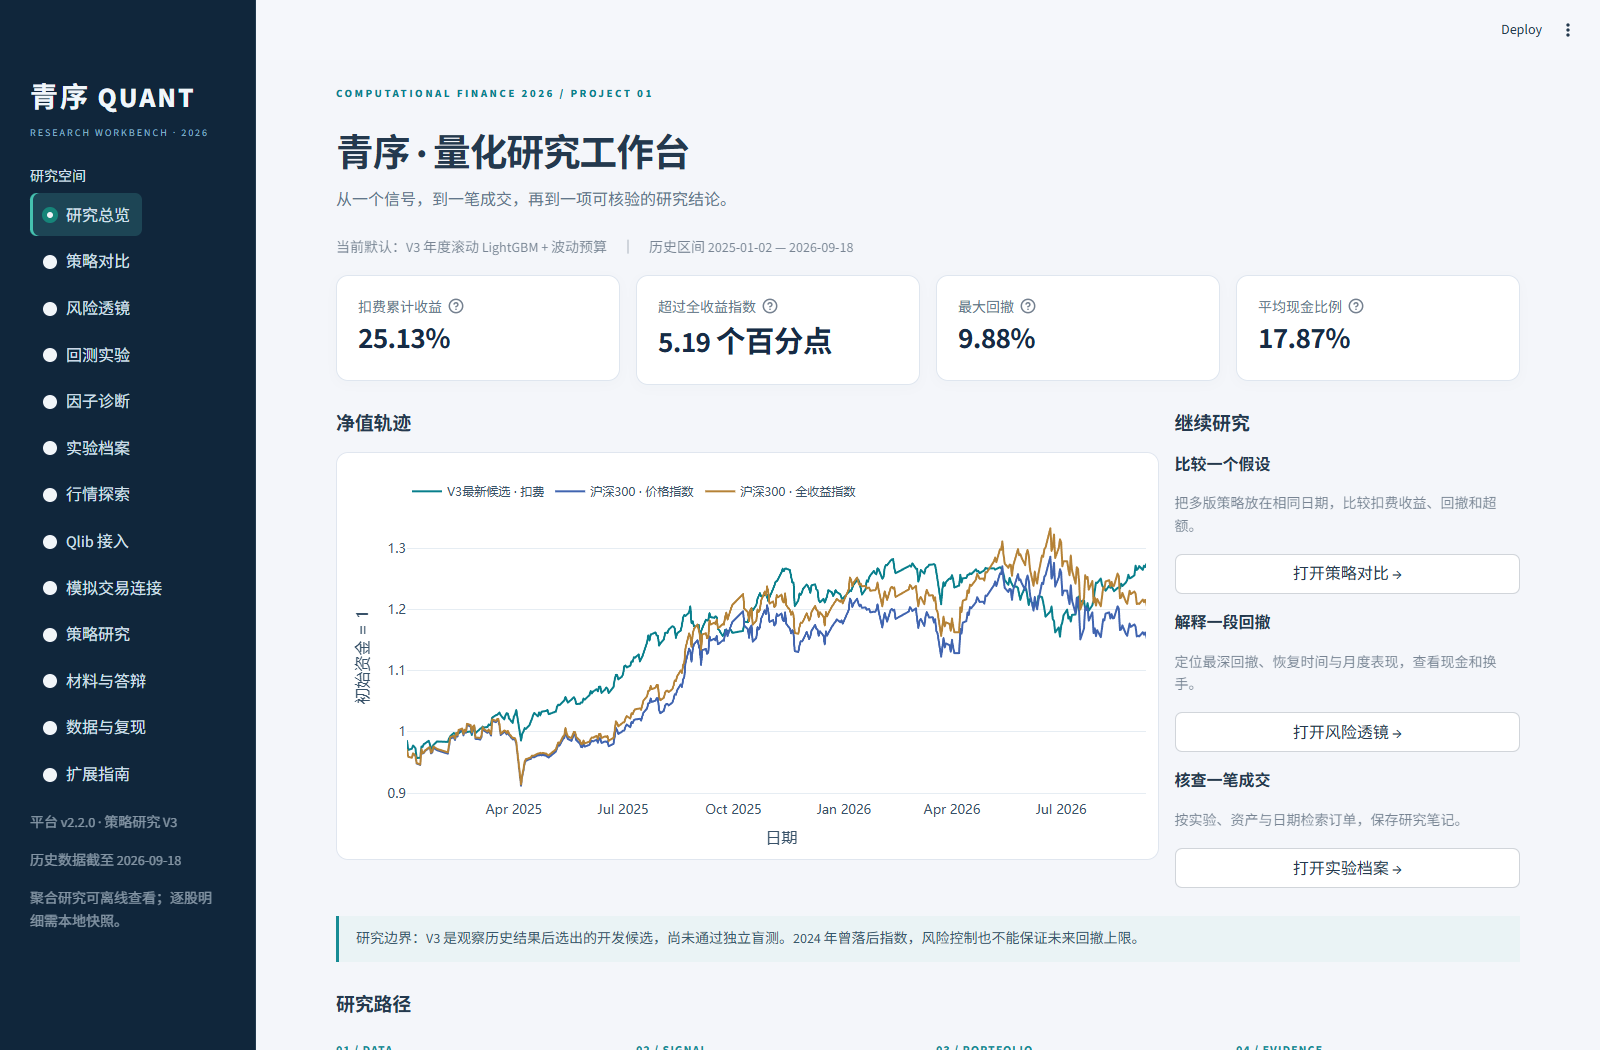
\includegraphics[width=.86\textwidth,height=57mm,keepaspectratio]{figures/ui-v4-overview.png}\end{center}
\page{3\quad 数据来源、质量与偏差}
\lead{固定选池日先于所有收益研究，历史缺失保留并计数。}
2019-12-31按当日成交额取符合主板代码、价格至少3元且有成交的前1,000只，并列按代码。没有使用今日仍上市名单，后来停止报价的原成员也保留。该池不包括2020年以后IPO，单日流动性选择偏向当时热点，结论不代表全A股或沪深300。
\begin{center}\begin{tabular}{lr}\toprule
核验项目 & 数量或结果\\\midrule
统一日线 / 日历交易日 & 1,656,599 / 1,690\\
完整股票×日历网格缺行 & 33,401\\
重复行情键 / 异常剔除 & 0 / 0\\
涨跌停价格缺失 / 最新有报价资产 & 48 / 956\\
每日估值记录 / 重复键 & 1,656,599 / 0\\
财务指标记录 / 单次返回最高行数 & 57,389 / 67（接口上限100）\\
行业历史区间 / 特征网格 & 1,432 / 1,690,000\\
原行情清单哈希 / 新研究清单哈希 & 3,006 / 2,073个文件通过\\\bottomrule
\end{tabular}\end{center}
\noindent\begin{tabularx}{\textwidth}{lX}\toprule
来源接口 & 字段、单位与用途\\\midrule
daily / adj\_factor & OHLC原价为元/股，vol源单位手转股；统一乘法复权供收益计算。\\
stk\_limit / trade\_cal & 原始涨跌停价和完整交易日历；缺限制价时不执行对应方向。\\
daily\_basic & total\_mv为万元，PE/PB为倍数，dv\_ttm与换手率为百分数；每日横截面。\\
fina\_indicator & ann\_date为公告日，end\_date为报告期；ROE为百分数，严格滞后使用。\\
index\_member\_all & 申万一级行业进出区间；未知或冲突标UNKNOWN，不将当前行业反填历史。\\
index\_daily / cn\_cpi & 沪深300价格/全收益指数；全国CPI月环比，按共同完整月份比较。\\\bottomrule
\end{tabularx}
\subsection*{复权、可得性与存储}
所有OHLC用\(P^{adj}_{i,t}=P^{raw}_{i,t}A_{i,t}/A_{i,ref}\)，每资产固定首个有效参考因子。原行情及V2研究缓存合计约1.63GB，包括原始缓存、标准数据、特征和模型分数。原始请求记录字段、日期与UTC下载时间，保存SHA-256；同请求可断点续拉。

历史行业未知比例约0.52\%，年度ROE平均覆盖约98.90\%（按每日合资格样本计算）。采用公告时点仍不能消除厂商事后修订，当前数据不是完整的逐版本财报库。保留此局限，不用“无未来函数”概括所有数据风险。

新增基准由Tushare指数目录确认H00300.CSI，再取全收益日线；另取510330.SH基金日线和复权因子，各1,690日。价格指数、全收益指数、ETF代理分开命名，未猜测或替代指数代码。
\page{4\quad 因子设计与标准接口}
\lead{12个因子覆盖不同假设，经济方向固定，负结果同样保留。}
记\(C,H,L,V\)为同尺度价格与股数，\(r_t=C_t/C_{t-1}-1\)。下表所有分数均为“越大越优先”的事前方向，缺失不补未来值。完整字段、窗口、失败情形和实现位置见\texttt{docs/FACTOR\_CARDS\_V2.md}。
\begin{center}\small\begin{tabular}{lll}\toprule
因子 & 公式与窗口 & 主要假设或风险\\\midrule
中期动量 & \(C_{t-20}/C_{t-60}-1\) & 跳过短期反转；趋势突变失效\\
短期反转 & \(-(C_t/C_{t-5}-1)\) & 超调修复；持续下跌失效\\
低波动 & \(-s(r,20)\) & 防御性；牛市可能落后\\
低振幅 & \(-\overline{(H-L)/C}_{20}\) & 日内风险；与低波动冗余\\
均线趋势 & \(C_t/\overline C_{20}-1\) & 趋势延续；震荡易反复\\
量能变化 & \(\log(\overline V_5/\overline V_{20})\) & 量能确认；方向可能不稳定\\
流动性 & \(-\overline{|r|/(C^{raw}V/10^6)}_{20}\) & 冲击较低；可能偏大盘\\
低换手 & \(-turnover\_rate\) & 降低拥挤；也可能缺乏交易\\
盈利收益率 & \(1/PE_{TTM},\ PE>0\) & 价值；亏损公司无定义\\
账面市值比 & \(1/PB,\ PB>0\) & 价值；资产质量有差异\\
股息率 & \(dv_{TTM}/100\) & 分红；历史分红不可保证\\
盈利质量 & 最新已公告年度\(ROE/100\) & 盈利能力；财报修订与滞后\\\bottomrule
\end{tabular}\end{center}
动量和反转要求整个价格窗口完整，波动等滚动统计要求完整观测；不将停牌前后压缩为相邻日。PE/PB非正为缺失，财报同公告、同报告期的冲突副本剔除，年度报表超过550日不再使用。建模时至少10个有效因子；剩余标准化缺值填0表示当日横截面中性值，不将缺失收益标签填0。
\subsection*{基础项与扩展项的关系}
原始20日动量、5日反转、20日低波动保留注册入口，可独立调窗口、诊断和回测。12因子研究采用固定配方，标准化等权平均为一个透明基线。中性化改变行业/市值暴露，不保证提高收益；本次没有因为某因子最终IC为负而翻转符号。
\subsection*{与Qlib和参考论文的关系}
参考Qlib Alpha158中的滞后、滚动量价表达以及训练/验证分离，复用LightGBM和scikit-learn模型实现。主策略12因子是明确列出的自定义研究集；独立Qlib表达式及Alpha158接入状态见第10页，\textbf{未将Qlib引擎替换进主成交账本}。CogAlpha论文采用代码形式的因子与LLM演化搜索，本项目借鉴可检查的因子表示，未开展大规模自动搜索。

\subsection*{实际横截面诊断}
已保存878个形成日的研究诊断；先按当日分数形成五组，再匹配下一开盘至20日后开盘标签。下表给出三个代表因子，完整12因子与有效人数见公开证据和独立因子页。
\begin{center}\small\begin{tabular}{lrrr}\toprule
因子 & 平均IC & 平均Rank IC & Q5--Q1平均20日收益\\\midrule
跳月动量 & $-0.0035$ & $-0.0161$ & $-0.0831\%$\\
5日反转 & $0.0176$ & $0.0187$ & $0.3264\%$\\
20日低波动 & $0.0378$ & $0.0722$ & $0.6377\%$\\\bottomrule
\end{tabular}\end{center}
负值不翻转；重叠20日标签不视为独立样本，也不连乘为可交易净值。
\page{5\quad 中性化、年度训练与8个候选}
\lead{因子处理按日进行；新模型只能使用当时已实现的标签。}
当日合资格因子按1\%/99\%截尾并用样本标准差标准化。对当日行业虚拟变量和对数市值回归取残差，再缩放为单位样本标准差。LightGBM同时输入12个标准化值和12个残差值，Ridge只输入12个残差值。
\[
z_{i,t}=\sum_g\alpha_{g,t}\mathbf1\{g_{i,t}=g\}+\beta_t\log MV_{i,t}+\epsilon_{i,t},\qquad n_{i,t}=\epsilon_{i,t}/s_t(\epsilon).
\]
每年第一次交易前一交易日形成新模型，训练此前3年。标签为次日开盘至20交易日后开盘收益的日横截面百分位减0.5，训练标签退出日必须严格早于模型形成日。整个下一年度使用该模型，到下一年才重训。
\begin{center}\small\begin{tabular}{lrr}\toprule
预测年度 & 训练观测数 & 最大标签退出日早于形成日\\\midrule
2023 & 654,563 & 已核验\\2024 & 645,816 & 已核验\\2025 & 636,902 & 已核验\\2026 & 634,716 & 已核验\\\bottomrule
\end{tabular}\end{center}
\begin{itemize}
\item 经济主题：价值（盈利/账面/股息）占50\%，ROE占25\%，低波动/低振幅占25\%。
\item Ridge：alpha=100，年度滚动重训，无最终期参数扫描。
\item LightGBM：250树，学习率0.03，15叶，最大深度5，最小叶500，L2=10，列采样0.8，种子20260921。
\item 固定融合：LightGBM百分位50\%、Ridge百分位25\%、经济主题百分位25\%。
\end{itemize}
四种信号各配稳定仓位及波动预算两种组合，共8个候选。稳定版本取消波动缩放和趋势折减；其他持仓、缓冲、上限及成交规则相同。2023--2024先记录验证结果及预选，然后再运行固定2025--2026区间。全部尝试保留在同一表。
\subsection*{与原建议的关系}
CNN需要有意义的局部邻接结构，简单排列的因子列没有天然邻接。V2已经保留小型MLP对照；本轮使用适合表格特征的树模型及线性基线，并未假定模型越复杂越好。年度训练减少长期冻结模型的陈旧性，但不能消除分布变化或过拟合。
\page{6\quad 组合、成交与账本核验}
\lead{每笔费用来自实际成交金额，模型只决定分数。}
每20个交易日调仓，目标50只。原持仓仍在前70名则优先保留，其余按分数补足，减少边界换手。先按波动率倒数构建权重，单股目标不超过4\%、行业目标不超过25\%；上限造成的余量留现金，不强制重新分配。

过去60日的候选组合收益估计年化波动率\(\hat\sigma\)。股票总预算为
\[
e_t=0.95\min\{1,0.20/\hat\sigma_t\}\times
\begin{cases}1,&CSI300_t\ge MA_{120,t},\\0.75,&\text{其他情况}.\end{cases}
\]
再应用个股与行业上限。所有估计截至形成日，次日开盘执行。风险估计中的少量历史缺价按0收益处理，是可低估风险的近似；实际缺价成交仍受阻。权重、波动和25\%回撤均为目标，不能保证市场变化后的实际风险。
\subsection*{成交与估值规则}
开盘按目标名义金额计算连续可分的复权单位，先卖后买，保留费用缓冲，现金不足同比缩减买单。涨停不买、跌停不卖、缺开盘或限制价不成交。每资产成交预算不超过此前20日平均成交额的1\%，超过时部分成交；这是事前容量代理，不是当日成交量的真实参与率保证。
\[
fee_t=0.001\,BuyNotional_t+0.0015\,SellNotional_t,\quad
Turnover_t=\frac{BuyNotional_t+SellNotional_t}{OpeningNAV_t}.
\]
买10bp、卖15bp是统一研究假设，不冒充历史法定税费。停牌持仓沿用最后已知收盘价并计数，连续缺失超过20个交易日保守计零；保留单位，恢复报价时重新估值，不虚构卖出。复权单位近似分红自动再投资，尚未模拟整手、完整分红现金或结算规则。
\subsection*{独立核验与扩展测试}
从成交逐笔重建现金与单位余额，再核对每日NAV、费用、换手与收益连乘。21个V3研究及压力运行全部通过，分别检查417、484或901个交易日。数值容差现金绝对\(10^{-6}\)元、相对\(10^{-10}\)。测试另覆盖手算、拆股连续性、独立Backtrader参考、未来扰动、公告滞后、中性化残差、无杠杆、部分成交及增量幂等。另以大面板逐项除法复现并修复本机可选NumExpr加速的错误常数结果，统一禁用该路径并重新生成全部研究；独立账本不能替代上游数值验证。最终测试与复算日志见验收清单。

\page{7\quad 失败、预选与开发后的候选}
\lead{更改研究目标不等于抹去原始失败。}
V1的20日动量、5日调仓长区间净收益为$-83.57\%$，最大回撤89.83\%；零费用独立重跑仍为$-75.16\%$。费用加回同成交路径得到$-58.12\%$，并非零费用独立策略，因为再投资路径不同。V2预选多因子在固定最终区间收益6.12\%，实现CPI目标但落后指数。
\subsection*{V3选择过程}
协议先写定8个候选与验证规则：2023--2024净收益、累计超额为正，最大回撤不超过25\%；先比较最差年度超额，再比较累计超额。价值质量主题稳定仓位排名第一，验证收益24.27\%、回撤9.16\%；但随后收益4.30\%，落后价格指数10.25个百分点。\textbf{这个预选失败不能被后续冠军替换。}
\begin{center}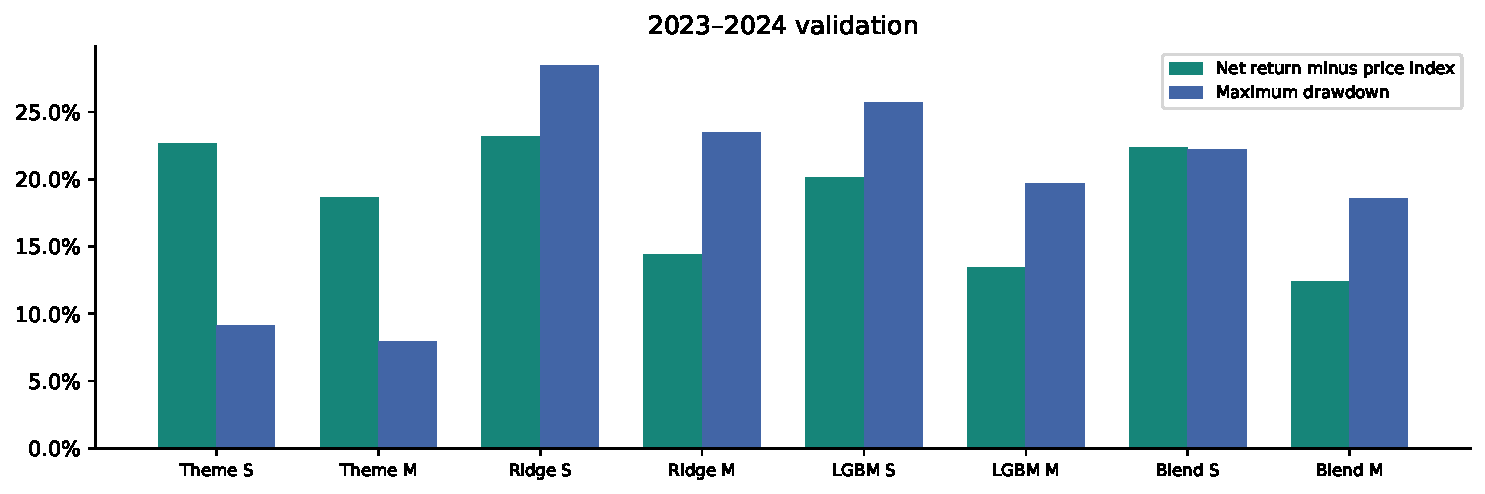
\includegraphics[width=.98\textwidth]{figures/validation.pdf}\end{center}
按用户要求进一步寻找能超过指数的历史候选，筛掉验证回撤超25\%的版本，再查看2025--2026超额。LightGBM稳定仓位虽然最终收益27.39\%，但验证回撤25.73\%，未作为默认。采用LightGBM波动预算版本，验证收益15.05\%、回撤19.70\%，最终收益25.13\%、回撤9.88\%。

以上是\textbf{开发后历史验收}，并非只有训练样本上的拟合收益，但也不属于全新盲测。决策文件保存preselected和selected两个字段，明确选择先后及8次候选规模。
\page{8\quad 固定区间的全候选与基准}
\lead{同一417日区间，策略费用已扣；基准名称及计息规则明确。}
\begin{center}\small\begin{tabular}{lrrr}\toprule
候选（稳定/波动预算） & 净收益 & 超价格指数 & 最大回撤\\\midrule
主题/稳定 & 4.30\% & -10.25\% & 9.13\%\\
主题/预算 & 5.68\% & -8.87\% & 8.76\%\\
Ridge/稳定 & 18.78\% & 4.23\% & 16.33\%\\
Ridge/预算 & 16.57\% & 2.02\% & 16.03\%\\
LGBM/稳定 & 27.39\% & 12.84\% & 9.75\%\\
LGBM/预算 & 25.13\% & 10.58\% & 9.88\%\\
融合/稳定 & 7.91\% & -6.64\% & 12.39\%\\
融合/预算 & 8.13\% & -6.42\% & 12.28\%\\\bottomrule\end{tabular}\end{center}
\begin{center}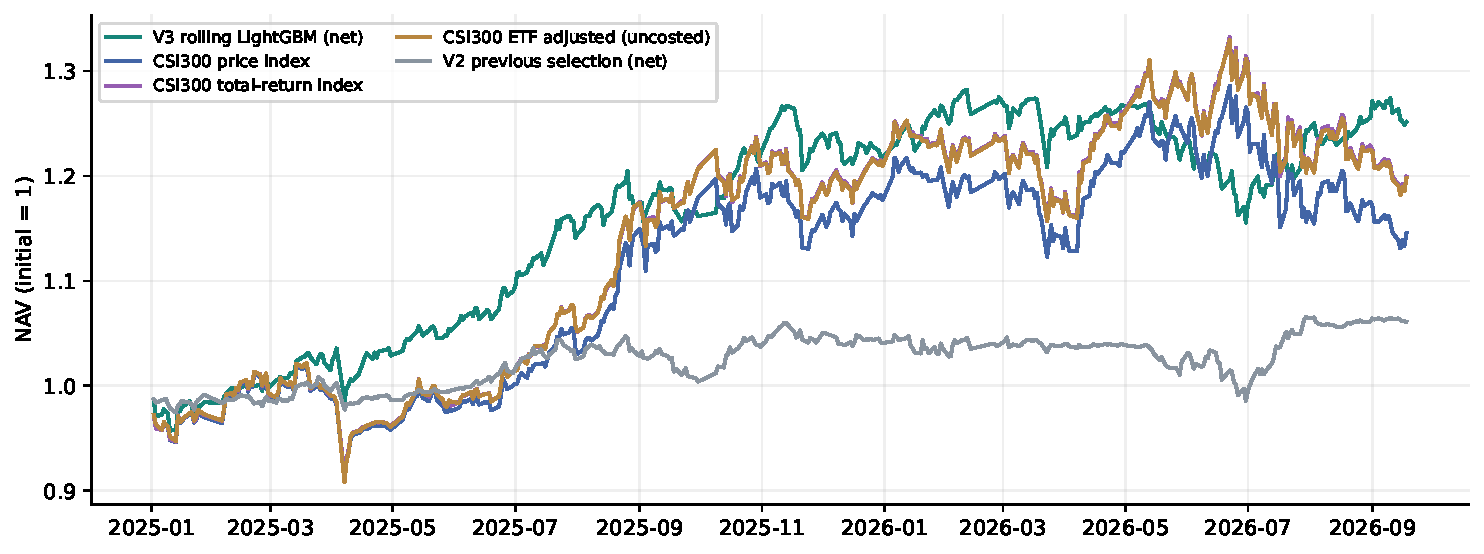
\includegraphics[width=.98\textwidth]{figures/nav.pdf}\end{center}
价格指数从前一交易日收盘归一化，累计14.55\%；全收益指数计红利再投资，累计19.94\%。策略同区间净收益25.13\%，相对全收益指数财富增长为$(1+25.13\%)/(1+19.94\%)-1\approx4.33\%$，与相差5.19个百分点是不同口径。

首次开盘起算价格指数收益14.64\%，结论不变。510330.SH复权未扣费代理收益19.82\%，另保留同开盘建仓扣买费的可交易近似；ETF不能改名为全收益指数。策略beta约0.30，年化跟踪误差15.60\%，信息比率0.292；落后阶段及主动净值回撤约18.41\%仍存在。
\page{9\quad 风险透镜与交互分析口径}
\lead{新增分析读取真实V3日账本，月收益与回撤恢复帮助解释风险。}
\begin{center}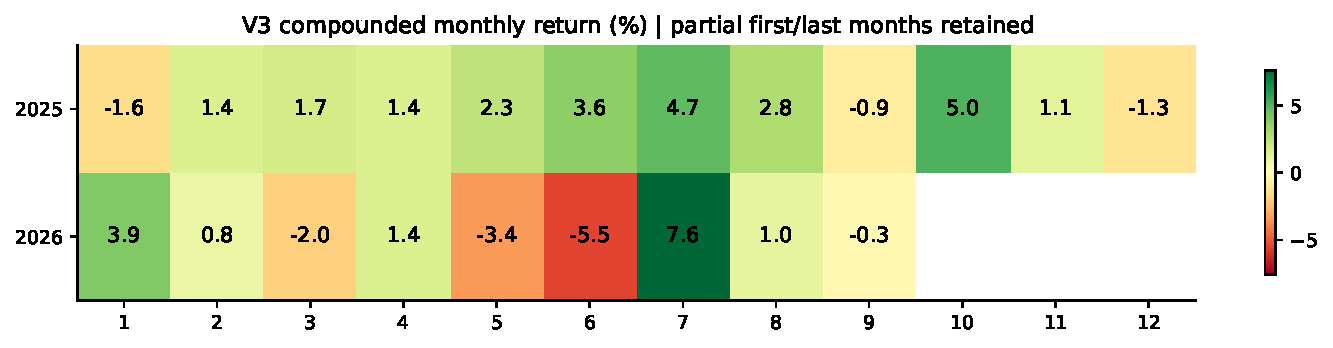
\includegraphics[width=.98\textwidth]{figures/v3_monthly.pdf}\end{center}
\begin{center}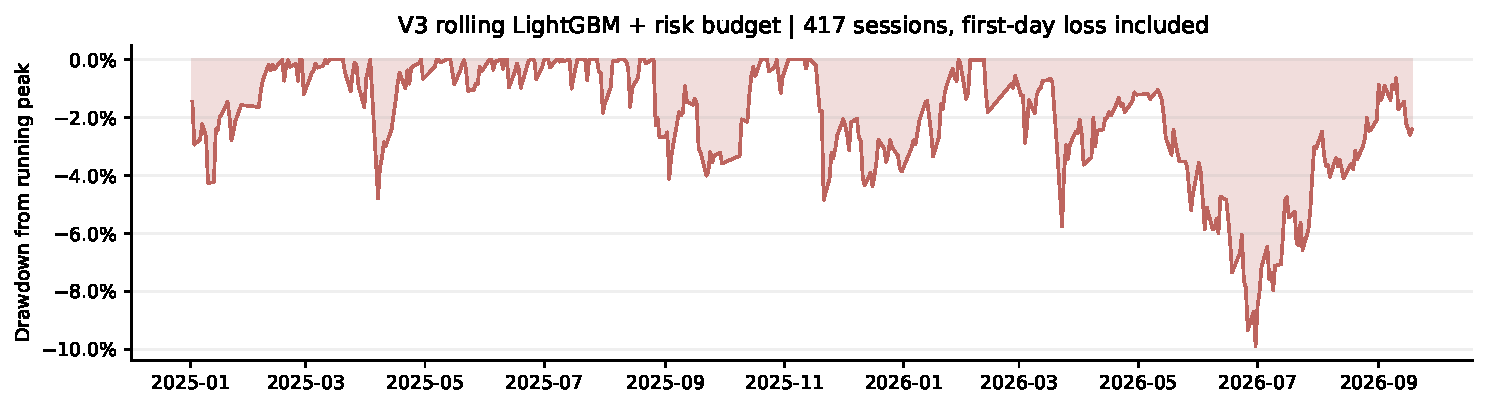
\includegraphics[width=.98\textwidth]{figures/v3_drawdown.pdf}\end{center}
\subsection*{日期、首日损益与回撤恢复}
同区间比较取交易日严格交集；内部缺日拒绝计算，不插值。区间第一日以此前收盘净值或明确初始资本作分母，保留首日损益；高水位包含初始资本。日期筛选是既有持仓路径的切片，不是从现金重新回测。未恢复回撤保留缺失恢复日期；无观测初始日期时不臆造峰值日期。
\subsection*{滚动风险与现金实验}
60日完整窗口计算复利收益、样本波动率和下行偏差，按252交易日年化；下行偏差以全部观察日作分母，目标为零。月历包括首尾不完整月份。静态资金分配采用$N_t^{mix}=wN_t+(1-w)$，现金零利息、不再平衡；输入通胀仅是购买力假设。该情景未重算规模对费用与成交容量的影响。费用占比为区间费用/期初净值，不等于零费用重跑的收益差。

\subsection*{既有压力检查保持不变}
双倍费用完整重跑净收益22.48\%，延迟一日27.31\%；2023起连续收益44.09\%、最大回撤19.70\%，2024仍落后价格指数7.28个百分点。延迟更好没有被用于修改默认参数；全部21组V3运行仍保留。
\page{10\quad 外部接入、验收与复现}
\subsection*{Qlib与同花顺连接状态}
Qlib 0.9.7在独立环境读取本地转换的数据；20股共33,754条日线，8个基础表达式与独立pandas计算逐项核对。共核对269,554个数值，有限值与缺失位置一致。另实际运行官方Alpha158的158项配置，158项至少有一个有限值，VWAP输入覆盖率100.0\%。这属于因子计算和数据接口验证，未训练Qlib交易策略，也未替换现有成交账本。

同花顺/SuperMind文件桥已完成：可导出历史权重与代码、导入模拟成交CSV并校验金额、保存本地回执。账号/API未连接，未收到真实账户文件，未提交任何订单；现金流核对不等于盈利。

\subsection*{课程要求与可检查的完成位置}
\begin{center}\small\begin{tabularx}{\textwidth}{lX}\toprule
要求 & 实现与证据\\\midrule
数据与因子 & 字段/复权/缺失/版本；原三因子、12因子卡及可配置窗口。\\
回测与指标 & 下一开盘、实际成交收费、现金/限制价/缺价、独立资金核对。\\
IC与分组 & 逐日横截面、有效样本数、先形成分组再匹配标签；负结果保留。\\
扩展与实践 & 历史行业市值中性化、风险预算、部分成交、增量审计、Qlib状态证据。\\
可用功能 & 版本回放、同区间对比、风险透镜、因子/行情、实验档案与笔记。\\
材料与复现 & 10页报告、20页Beamer/PowerPoint、逐页讲稿、源码与哈希。\\\bottomrule
\end{tabularx}\end{center}
主环境102项测试通过，1项可选Qlib集成测试因无依赖跳过；独立Qlib环境5项通过，包含被跳过的真实引擎集成项；V3原研究21个账本核对和独立环境复算保留。工程检查验证计算实现，不能替代未来市场泛化证明。
\subsection*{运行与来源}
本机双击launch.cmd。新环境按REPRODUCE\_V4安装固定依赖，运行自动化测试和合成示例；无凭据先查看公开真实证据，补足合法原始数据后再运行训练。原V3研究目录防覆盖；改变假设必须保存新实验。材料、指标、Git标签v2.2.0和数据身份共同定位交付。

课程依据CF2026\_Project1.pdf（19页）；金融基准采用中证与Tushare官方定义。Qlib官方代码/文档及接入版本用于表达式核查；来源与连接状态详见仓库文档。CogAlpha仅借鉴代码式因子表示，未声称复刻整篇方法。
\subsection*{提交边界}
当前候选经历史复核后选择，不是独立盲测。固定2019池、财报修订、历史行业重构和缺失估值限制外推；复权连续单位尚不覆盖整手、完整分红现金、结算与真实盘口。原始缓存和Token不公开；文件桥不代表账户接通或下单。提交前填写组员姓名、学号并按教师要求命名；材料已准备，评分与课程提交状态由实际验收决定。
\end{document}
